\documentclass[sigconf]{acmart}

\settopmatter{printacmref=false}
\renewcommand\footnotetextcopyrightpermission[1]{}
\pagestyle{plain}

\AtBeginDocument{%
  \providecommand\BibTeX{{\normalfont B\kern-0.5em{\scshape i\kern-0.25em b}\kern-0.8em\TeX}}%
}

\begin{document}

\title{Unsupervised Tumor/Normal Classification of Kidney Renal Clear Cell Carcinoma from DNA Methylation Data}

\author{Tyrone C. Mariano}
\affiliation{%
  \institution{Department of Computer Science, University of the Philippines Diliman}
  \city{Quezon City}
  \country{Philippines}
}
\email{tcmariano@up.edu.ph}

\author{Jhoirene B. Clemente}
\affiliation{%
  \institution{Department of Computer Science, University of the Philippines Diliman}
  \city{Quezon City}
  \country{Philippines}
}
\email{jbclemente@up.edu.ph}

\renewcommand{\shortauthors}{Mariano and Clemente}

\begin{abstract}
Supervised tumor/normal classifiers trained on DNA methylation data routinely achieve near-perfect discrimination, but they depend on ground-truth labels that are expensive to obtain in many clinical settings. We ask whether an entirely unsupervised pipeline, using unlabeled methylation data, can approach the same performance for kidney renal clear cell carcinoma (KIRC). Using TCGA-KIRC Illumina 450K methylation profiles, we compare the performance of Support Vector Machine (SVM) and Random Forest (RF) trained on pseudo-labels and on ground truth labels. The pseudo-labels were generated using the cluster assignments from K-means, hierarchical, and Gaussian mixture clustering of dimensionally reduced data from Principal Component Analysis (PCA) and Uniform Manifold Approximation and Projection (UMAP). PCA decisively outperforms UMAP (mean Adjusted Rand Index, ARI, of 0.79 versus 0.07 across different configurations), and the automatically selected best configuration (KMeans on 112 principal components) yields classifiers trained on pseudo-labels within 0.005 AUC of classifiers trained on ground truth (SVM: 0.995 vs.\ 1.000; RF: 0.997 vs.\ 0.999), reproduced under 5-fold cross-validation. Most notably, we show that the cluster features' ARI is strongly negatively correlated with the pseudo-label/ground-truth AUC gap ($r=-0.93$ for SVM, $r=-0.94$ for RF), letting ARI serve as a validation signal wherever some labeled reference data is available; we further show, by direct test, that fully label-free metrics (silhouette, Davies--Bouldin) cannot substitute for ARI in this role. These AUC results are benchmarked with published methylation-based pan-cancer diagnostic experiments and suggest that unsupervised pseudo-labeling is a viable substitute for supervision in KIRC tumor/normal classification, given some reference ground truth to validate it.
\end{abstract}

% \begin{CCS2012}
% <concept>
% <concept_id>10010147.10010257.10010258.10010259.10010263</concept_id>
% <concept_desc>Computing methodologies~Cluster analysis</concept_desc>
% <concept_significance>500</concept_significance>
% </concept>
% <concept>
% <concept_id>10010147.10010257.10010293.10010294</concept_id>
% <concept_desc>Computing methodologies~Supervised learning by classification</concept_desc>
% <concept_significance>500</concept_significance>
% </concept>
% <concept>
% <concept_id>10010147.10010257.10010293.10010296</concept_id>
% <concept_desc>Computing methodologies~Unsupervised learning</concept_desc>
% <concept_significance>500</concept_significance>
% </concept>
% <concept>
% <concept_id>10010405.10010481.10010485</concept_id>
% <concept_desc>Applied computing~Bioinformatics</concept_desc>
% <concept_significance>300</concept_significance>
% </concept>
% \end{CCS2012}

\ccsdesc[500]{Computing methodologies~Cluster analysis}
\ccsdesc[500]{Computing methodologies~Unsupervised classification}
\ccsdesc[300]{Applied computing~Bioinformatics}

\keywords{DNA methylation, kidney renal clear cell carcinoma, unsupervised learning, pseudo-labeling, clustering, dimensionality reduction, PCA, UMAP}

\maketitle

\section{Introduction}
\label{sec:intro}

DNA methylation is among the most reliable molecular signals for distinguishing tumor from adjacent normal tissue as it is more stable than gene expression. Moreover, genome-wide array platforms such as the Illumina 450K make it cheap to profile at scale. Prior pan-cancer studies report tumor/normal discrimination AUCs above 0.99 using only a handful of CpG sites \cite{ding2019integrative, liu2019dna}. Kidney renal clear cell carcinoma (KIRC) methylation studies have largely moved past this diagnostic question and now target the harder problem of prognosis, where AUCs of 0.75--0.82 are typical \cite{tang2020novel}. This suggests that KIRC tumor/normal separability is already near a performance ceiling in the \emph{supervised} setting.

The supervised setting, however, assumes clean, verified tumor/normal labels for every training sample, an assumption that does not hold in many practical scenarios, such as newly collected cohorts awaiting pathological confirmation, federated data where label sharing is restricted, or exploratory analyses of public repositories with inconsistent annotation. This motivates an unsupervised alternative: reduce the dimensionality of the methylation profile, cluster the reduced representation into two groups, treat cluster membership as a \emph{pseudo-label}, and train a standard classifier on those pseudo-labels.

This raises three practical questions that we address directly. First, does dimensionality-reduction choice matter, and can it be decided empirically rather than by convention? Second, how close can a classifier trained on pseudo-label get to a classifier trained on ground-truth labels, and does that gap hold up under resampling? Third, does clustering quality itself \emph{predict} how trustworthy the resulting pseudo-label classifier will be, and can that prediction be made using only label-free, internal clustering metrics, or does it still require some reference ground truth?

Our main contributions are: (1) a rigorous unsupervised classification pipeline for TCGA-KIRC methylation data with an automatic (non-hand-picked) selection of the best clustering configuration for pseudo-label generation; (2) a decisive empirical comparison showing PCA vastly outperforms UMAP as the dimensionality-reduction front end for this task (mean ARI 0.79 vs.\ 0.07); (3) evidence that classifiers trained on pseudo-label are nearly interchangeable with classifiers trained on ground truth labels (AUC gap $<0.005$), which was confirmed under 5-fold patient-grouped cross-validation; and (4) a novel finding that clustering ARI strongly predicts the pseudo-label/ground-truth AUC gap ($r=-0.93$ to $-0.94$), together with a direct test showing that fully label-free internal metrics (silhouette, Davies--Bouldin) cannot substitute for ARI in this role -- an important caveat for anyone hoping to validate an unsupervised pipeline with zero reference labels.

\section{Materials and Methods}

\subsection{Data and Preprocessing}
We used Illumina 450K DNA methylation profiles for KIRC from The Cancer Genome Atlas (TCGA), obtained via Xena Hub, together with matched clinical tumor/normal annotations. Probes with more than 1\% missing values across samples were dropped, leaving 371{,}082 probes. Samples were split into training and holdout sets using a \emph{patient-grouped} split (\texttt{GroupShuffleSplit}, 60/40, seed fixed): patients contribute matched tumor and normal samples, so a naive sample-level split leaks patient identity across the train/holdout boundary and inflates downstream AUC. Grouping by the first 12 characters of the TCGA barcode (patient identifier) guarantees zero patient overlap. The resulting training set contains 285 samples (193 tumor, 92 normal) and the holdout set contains 198 samples (130 tumor, 68 normal), spanning 191 unique training patients. All feature scaling, dimensionality reduction, and clustering models are fit exclusively on the training set and only applied to the holdout.

\subsection{Dimensionality Reduction}
We compared two dimensionality-reduction methods as a preliminary step before clustering: PCA and UMAP \cite{mcinnes2018umap}, each evaluated at three settings: 2 components, 3 components, and a systematically chosen ``optimal'' number of components. For PCA, the optimal dimensionality was the smallest $n$ such that the cumulative explained variance reached 80\% ($n=112$); we note that we obtain this $n$ by searching over the full feasible rank and adding an explicit failure guard. For UMAP, optimal dimensionality was chosen by sweeping $n \in \{5, 15, 30\}$ and selecting the value maximizing the silhouette score of the resulting embedding ($n=30$).

\subsection{Clustering and Pseudo-Label Generation}
At each dimensionality, we ran three clustering algorithms with two imposed clusters ($K=2$): KMeans, agglomerative (hierarchical) clustering, and a Gaussian Mixture Model (GMM) \cite{jain2010clustering}. Because cluster indices (0/1) are arbitrary, we align each clustering's label direction to ground truth by majority vote before scoring. We additionally include a raw-feature (no dimensionality reduction) KMeans and hierarchical baseline for reference. Full-covariance GMM in the 112-dimensional ``optimal'' setting fit the training data well (ARI 0.889) but collapsed to a single cluster on holdout data (ARI 0.000); we therefore restrict high-dimensional GMM to diagonal covariance. Clustering quality is scored against ground truth using the Adjusted Rand Index (ARI) \cite{hubert1985comparing}, it is a chance-corrected, label-permutation-invariant agreement metric. We additionally verify with label-free silhouette and Davies--Bouldin scores to test
separately (Section 3.5) whether these internal, ground-truth-free
metrics can serve as a substitute for ARI. Among all configurations restricted to those that support out-of-sample prediction (i.e., excluding hierarchical clustering, which has no \texttt{predict()} method), the best-ARI configuration is selected \emph{automatically}, saved as \texttt{joblib} file, and will be used for downstream analyses.


\subsection{Classification}
For the selected pseudo-labels, and separately for ground truth, we train an RBF-kernel SVM and a Random Forest (100 trees) \cite{cortes1995support, breiman2001random} on the training set and evaluate ROC AUC on the untouched holdout set. This lets us directly compare a classifier trained on pseudo-label or ``pseudo-label classifier'' against a classifier  trained on ground-truth labels or ``ground-truth classifier''. Both settings are trained on identical features and only differs in the target feature.

\subsection{Cross-Validation Robustness Analysis}
\label{sec:cvmethods}
To test whether our point-estimate results are stable, and to test the ARI/AUC-gap relationship across a wide range of clustering qualities, we ran 5-fold patient-grouped cross-validation (\texttt{GroupKFold}). Within each fold, the scaler, PCA, and clustering model are \emph{refit from scratch} on that fold's training portion, never reusing a globally fit model, to avoid cross-fold leakage. We evaluated six configurations pairing PCA at $n\in\{2,3,112\}$ with GMM (full covariance) or KMeans -- the latter directly validates, under resampling, the same configuration (PCA(112)$\times$KMeans) that Section~\ref{sec:autoselect} selects as the deployed model. We added a seventh, deliberately poor arm, UMAP(30)$\times$Hierarchical -- the worst-performing configuration already found on the full training split (Table~\ref{tab:ari}, ARI $=0.018$) -- to widen the observed ARI range beyond the narrow, near-ceiling band the six well-tuned arms share, so the ARI-vs-AUC-gap relationship (Section~\ref{sec:aritrust}) has room to be tested. Its classifier is trained on the same UMAP(30) features used for clustering, keeping the pipeline structurally identical to the six good arms.

\section{Results}

\subsection{PCA Decisively Outperforms UMAP}
Figure~\ref{fig:pca_umap} and Table~\ref{tab:ari} compare PCA and UMAP across all nine (dimensionality reduction $\times$ clustering algorithm) configurations. PCA achieves a higher ARI than UMAP in \emph{every single configuration} (mean ARI 0.79 vs.\ 0.07). The best PCA configurations are KMeans at $n=112$ and hierarchical at $n=3$ (both ARI $=0.876$); the best UMAP configuration (hierarchical, $n=2$, ARI $=0.126$) does not come close. A raw-feature (no reduction) KMeans baseline is degenerate (ARI $=-0.007$), confirming dimensionality reduction is necessary, not merely helpful, for KMeans here. We attribute this to the nature of the tumor/normal signal: a broad, global shift in methylation, which PCA's variance-maximizing objective captures well but UMAP's local-neighborhood-preserving objective does not.

\begin{figure}[t]
\centering
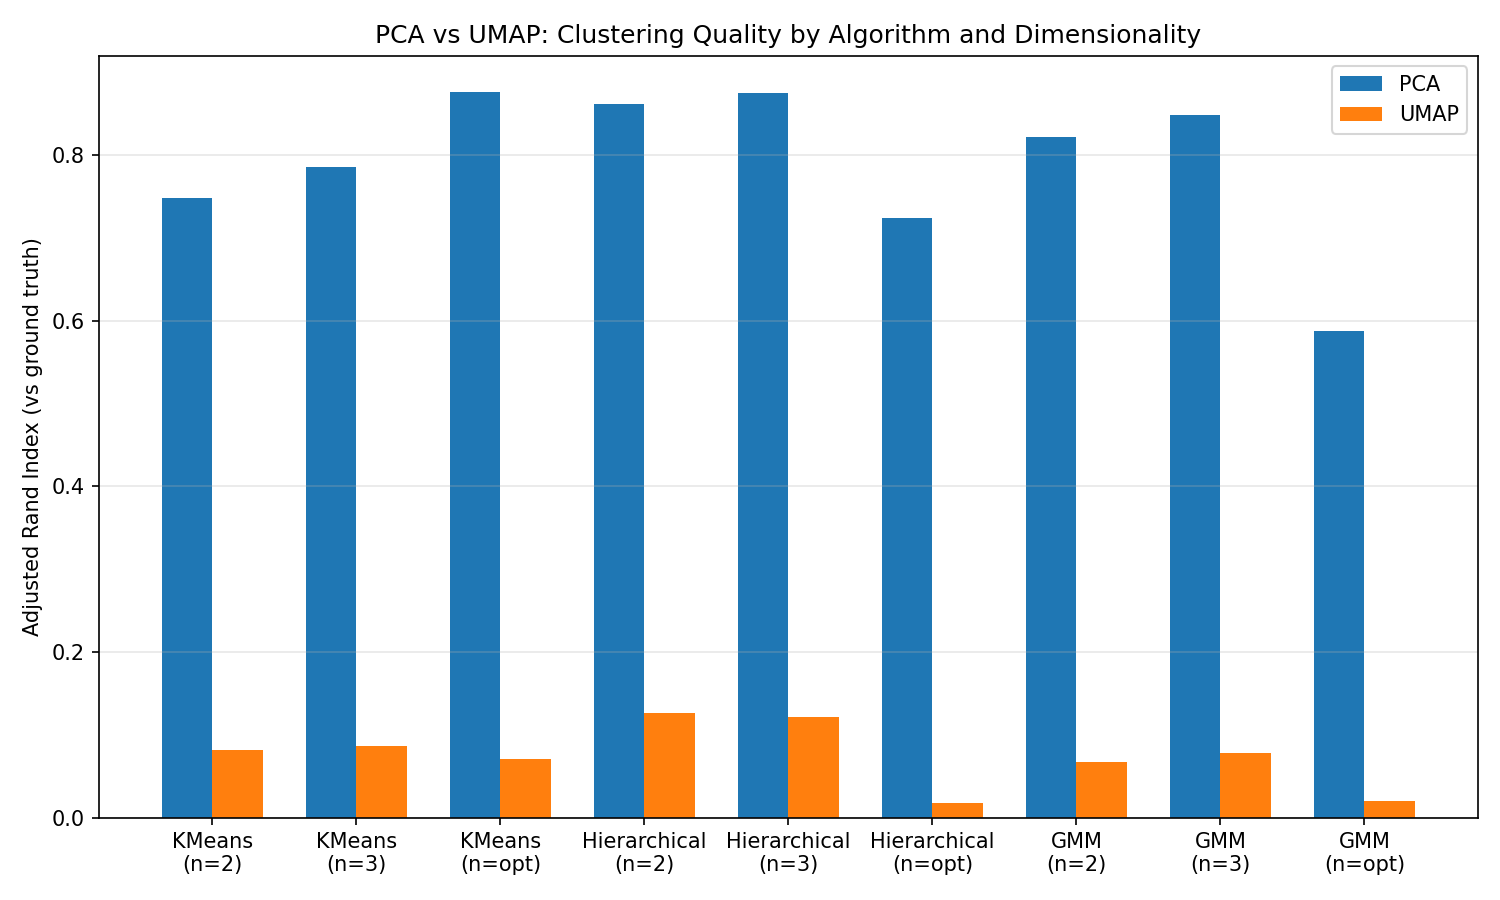
\includegraphics[width=\columnwidth]{images/pca_vs_umap_comparison.png}
\caption{ARI for PCA vs.\ UMAP across three clustering algorithms and three dimensionalities. PCA wins in every configuration tested.}
\label{fig:pca_umap}
\Description{Bar chart comparing Adjusted Rand Index for PCA and UMAP across KMeans, Hierarchical, and GMM clustering at 2, 3, and optimal dimensionality, showing PCA consistently higher.}
\end{figure}

\begin{table}[t]
\caption{Clustering ARI against ground truth: PCA vs.\ UMAP space.}
\label{tab:ari}
\resizebox{\columnwidth}{!}{%
\begin{tabular}{lcccccc}
\toprule
 & \multicolumn{3}{c}{PCA} & \multicolumn{3}{c}{UMAP} \\
Algorithm & $n=2$ & $n=3$ & opt.\ & $n=2$ & $n=3$ & opt.\ \\
\midrule
KMeans        & 0.749 & 0.786 & \textbf{0.876} & 0.082 & \textbf{0.086} & 0.071 \\
Hierarchical  & 0.862 & \textbf{0.876} & 0.724 & \textbf{0.126} & 0.122 & 0.018 \\
GMM (diag.)   & 0.822 & \textbf{0.848} & 0.588 & 0.067 & \textbf{0.078} & 0.020 \\
\bottomrule
\end{tabular}}
\end{table}

\subsection{Automatic Selection and Pseudo-Label Classification}
\label{sec:autoselect}
Restricting to configurations that support out-of-sample prediction, our pipeline automatically selects KMeans at the optimal PCA dimensionality ($n=112$, ARI $=0.876$) as the deployable configuration. Figure~\ref{fig:roc} shows ROC curves on the holdout set for SVM and RF trained on this pseudo-label versus trained on ground truth, using identical PCA-reduced features. The pseudo-label and ground-truth classifiers are nearly indistinguishable: SVM achieves AUC 0.995 (pseudo-label) versus 1.000 (ground truth), and RF achieves 0.997 versus 0.999 -- a gap under 0.005 AUC in both cases.

\begin{figure}[t]
\centering
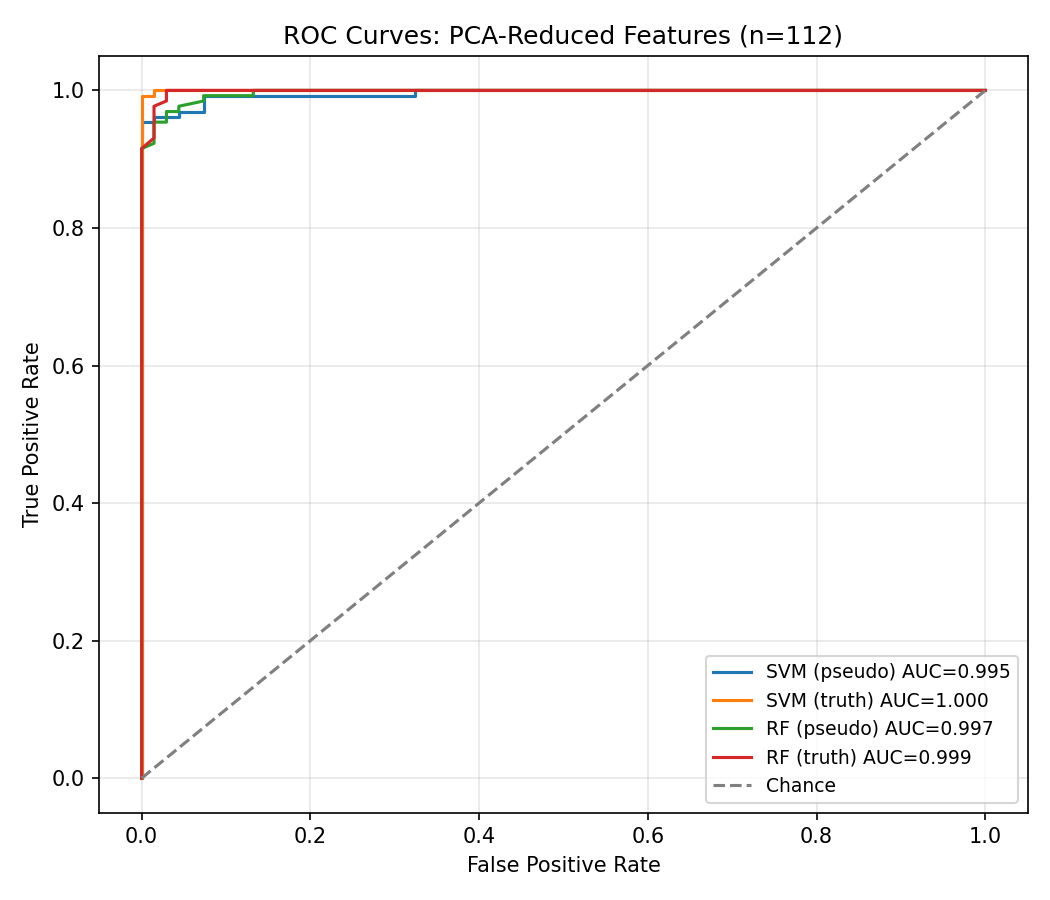
\includegraphics[width=\columnwidth]{images/roc_curves_pca_validation.png}
\caption{Holdout ROC curves: classifiers trained on pseudo-labels closely track classifiers trained on ground truth.}
\label{fig:roc}
\Description{ROC curves for SVM and Random Forest trained on pseudo-labels versus ground truth, all curves close to the top-left corner with AUC between 0.99 and 1.00.}
\end{figure}

\subsection{Cross-Validation Confirms Robustness}
Table~\ref{tab:cv} reports 5-fold patient-grouped cross-validation results (mean $\pm$ std) for the seven configurations defined in Section~\ref{sec:cvmethods}. Across all six well-chosen PCA$\times$\{GMM,KMeans\} configurations, ARI stays well above chance and both classifiers retain AUC $\geq 0.98$ with low fold-to-fold variance, confirming the single-split results above are not an artifact of a favorable split. Most importantly, \textbf{PCA(112)$\times$KMeans -- the actual deployed configuration -- reproduces its single-split ARI closely under resampling}: CV ARI $=0.850\pm0.027$, versus $0.876$ on the full single split (Section~\ref{sec:autoselect}) and $0.8245$ on the held-out set (Section~\ref{sec:generalization}), confirming the CV protocol validates the same model actually deployed, not merely a related one. The UMAP(30)$\times$Hierarchical arm behaves very differently: ARI stays consistently low (mean $0.117 \pm 0.009$), and the pseudo-label classifier AUC degrades correspondingly (SVM: $0.589 \pm 0.080$; RF: $0.593 \pm 0.040$) while the ground-truth classifier on the identical features stays high (SVM: $0.934\pm0.037$; RF: $0.948\pm0.047$) -- isolating the degradation to pseudo-label quality itself, not the underlying features. Figure~\ref{fig:boxplot} visualizes this contrast.

\begin{table}[t]
\caption{5-fold patient-grouped CV: ARI and AUC (mean $\pm$ std). The last row's classifier is trained on the same UMAP(30) features used to generate its (deliberately poor) pseudo-label (Section~\ref{sec:cvmethods}).}
\label{tab:cv}
\resizebox{\columnwidth}{!}{%
\begin{tabular}{lccccc}
\toprule
Config.\ (DR $\times$ Alg.) & ARI & SVM (ps.) & SVM (gt.) & RF (ps.) & RF (gt.) \\
\midrule
PCA(2)$\times$GMM      & 0.852$\pm$.019 & 0.991$\pm$.012 & 0.993$\pm$.008 & 0.981$\pm$.026 & 0.987$\pm$.015 \\
PCA(3)$\times$GMM      & 0.865$\pm$.043 & 0.992$\pm$.008 & 0.993$\pm$.009 & 0.983$\pm$.023 & 0.992$\pm$.007 \\
PCA(112)$\times$GMM    & 0.853$\pm$.030 & 0.984$\pm$.014 & 1.000$\pm$.000 & 0.999$\pm$.002 & 0.999$\pm$.001 \\
PCA(2)$\times$KMeans   & 0.724$\pm$.086 & 0.987$\pm$.015 & 0.993$\pm$.008 & 0.983$\pm$.016 & 0.987$\pm$.015 \\
PCA(3)$\times$KMeans   & 0.727$\pm$.085 & 0.988$\pm$.018 & 0.993$\pm$.009 & 0.991$\pm$.009 & 0.992$\pm$.007 \\
PCA(112)$\times$KMeans & \textbf{0.850$\pm$.027} & 0.985$\pm$.014 & 1.000$\pm$.000 & 0.999$\pm$.002 & 0.999$\pm$.001 \\
UMAP(30)$\times$Hierarchical & 0.117$\pm$.009 & 0.589$\pm$.080 & 0.934$\pm$.037 & 0.593$\pm$.040 & 0.948$\pm$.047 \\
\bottomrule
\end{tabular}}
\end{table}

\begin{figure}[t]
\centering
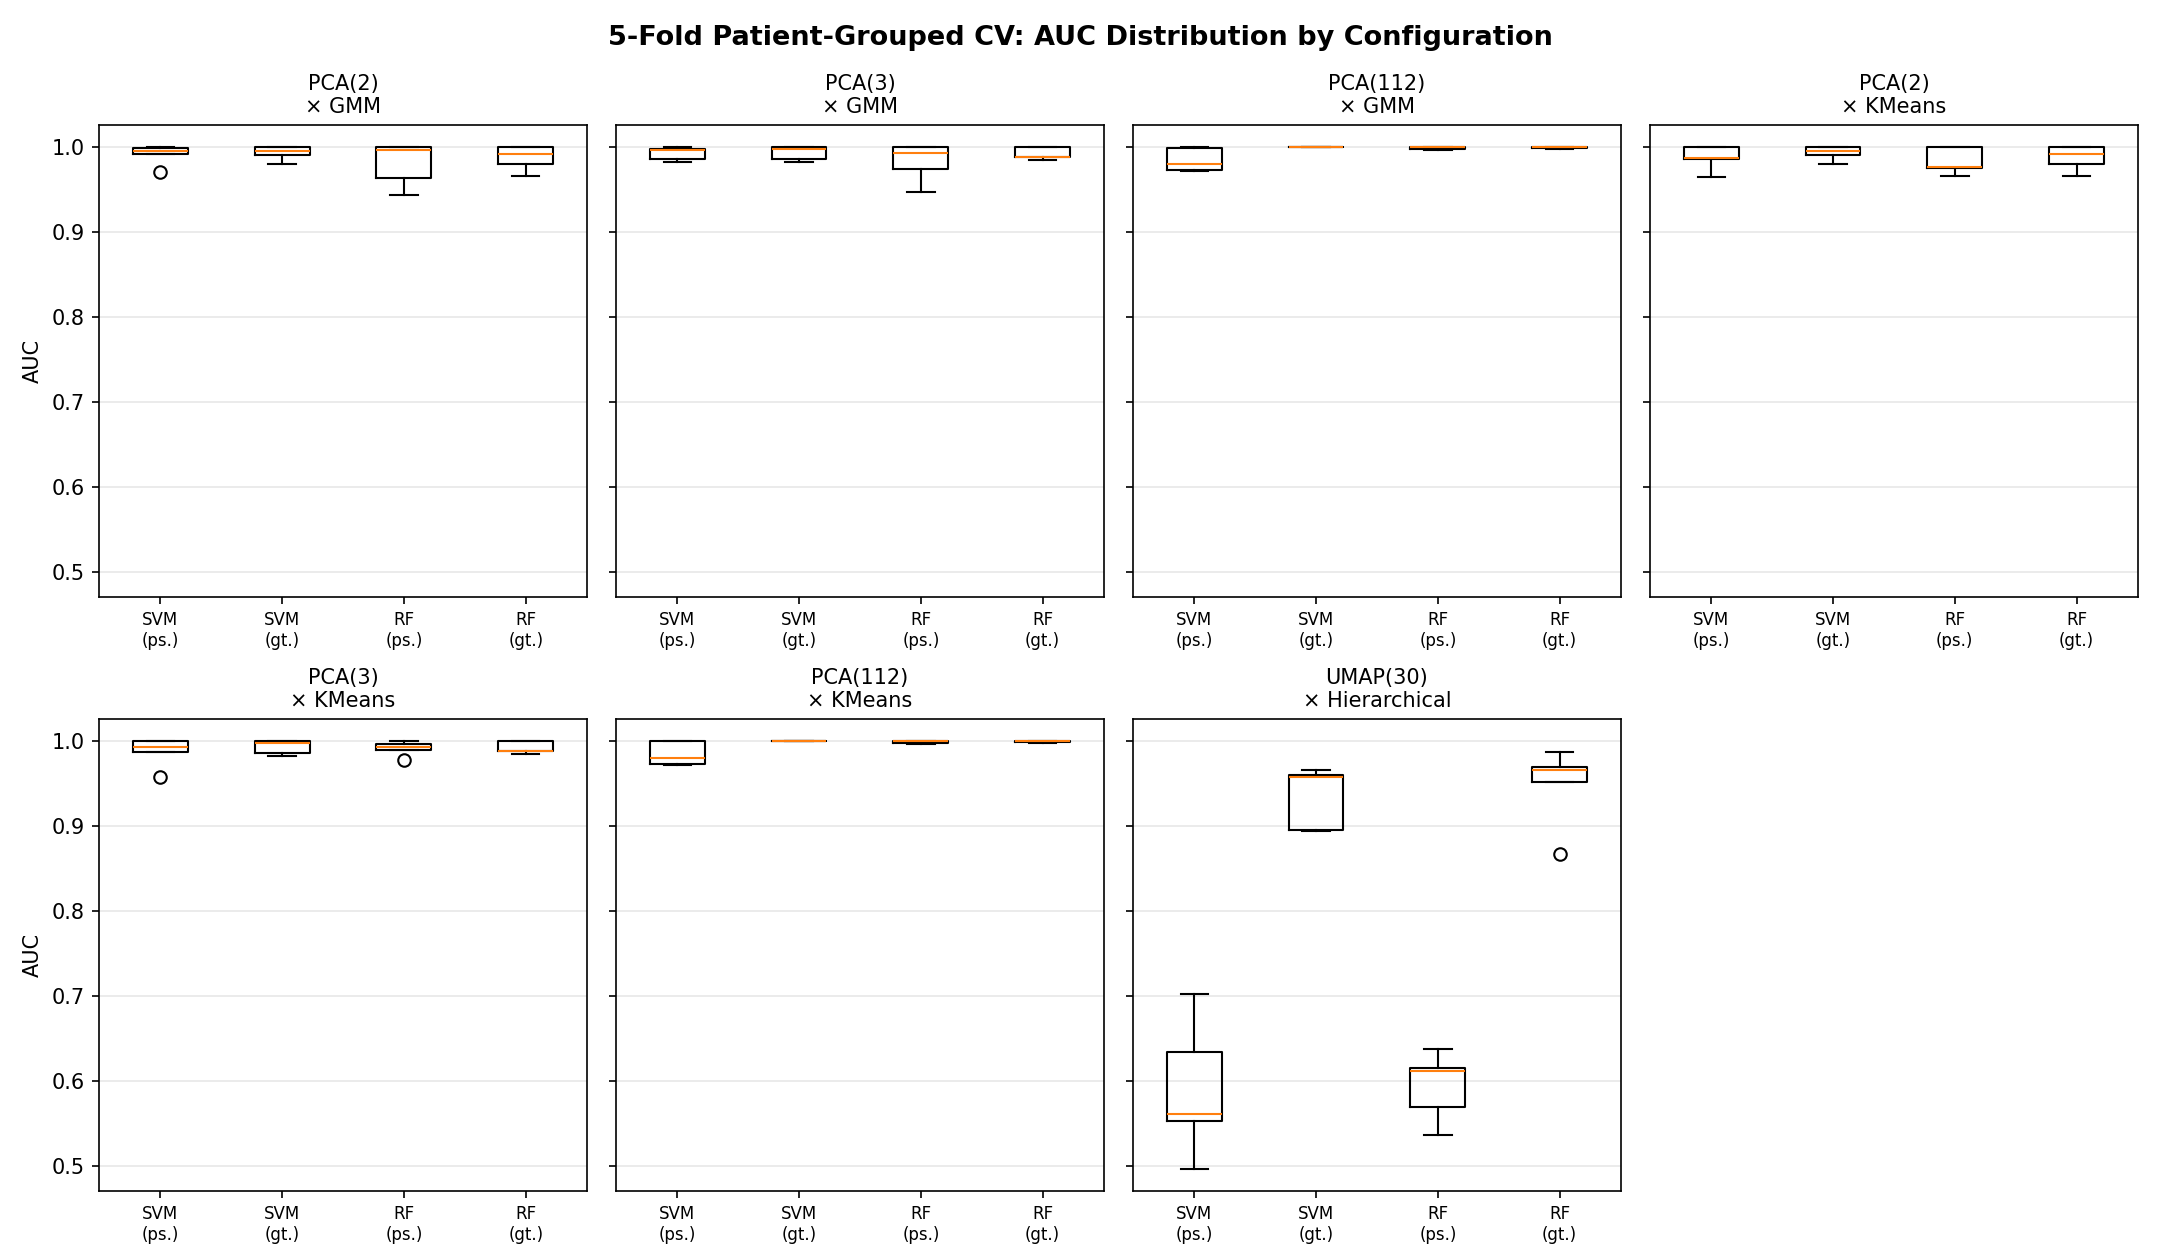
\includegraphics[width=\columnwidth]{images/cv_auc_boxplot.png}
\caption{Cross-validated AUC by configuration (panel titles give the DR $\times$ algorithm pairing; see Table~\ref{tab:cv}). The six PCA$\times$\{GMM,KMeans\} configurations (first six panels) are high and tight, including PCA(112)$\times$KMeans, the actual deployed model; the deliberately poor UMAP(30)$\times$Hierarchical configuration (last panel) is consistently low, with a clear separation between the ground-truth and pseudo-label boxes.}
\label{fig:boxplot}
\Description{Boxplots of AUC across cross-validation folds for seven configurations, arranged in a grid, showing narrow high-AUC boxes for the six PCA-based configurations and a consistently lower pair of boxes (pseudo-label) versus a higher pair of boxes (ground truth) for the deliberately poor UMAP-Hierarchical configuration.}
\end{figure}

\subsection{Clustering Quality Predicts Classifier Trustworthiness}
\label{sec:aritrust}
Our central and most novel finding concerns the relationship between clustering quality and pseudo-label classifier reliability. The poor-clusterer arm gives us per-fold (ARI, AUC-gap) pairs spanning a wide range of clustering quality, rather than the narrow, near-ceiling range the six good configurations alone would produce. Figure~\ref{fig:gap} plots the clustering ARI against the absolute gap between the pseudo-label and ground-truth classifiers' AUC, one mean point per configuration and model. The underlying relationship, computed across all 35 individual fold-level observations, is strongly negative: Pearson $r=-0.93$ for SVM and $r=-0.94$ for RF. In other words, \emph{the better the clustering agrees with (unseen) ground truth, the smaller the performance penalty from training on its pseudo-labels instead} -- detectable using only clustering-internal information, and holding across two different clustering algorithms rather than being an artifact of one.

\begin{figure}[t]
\centering
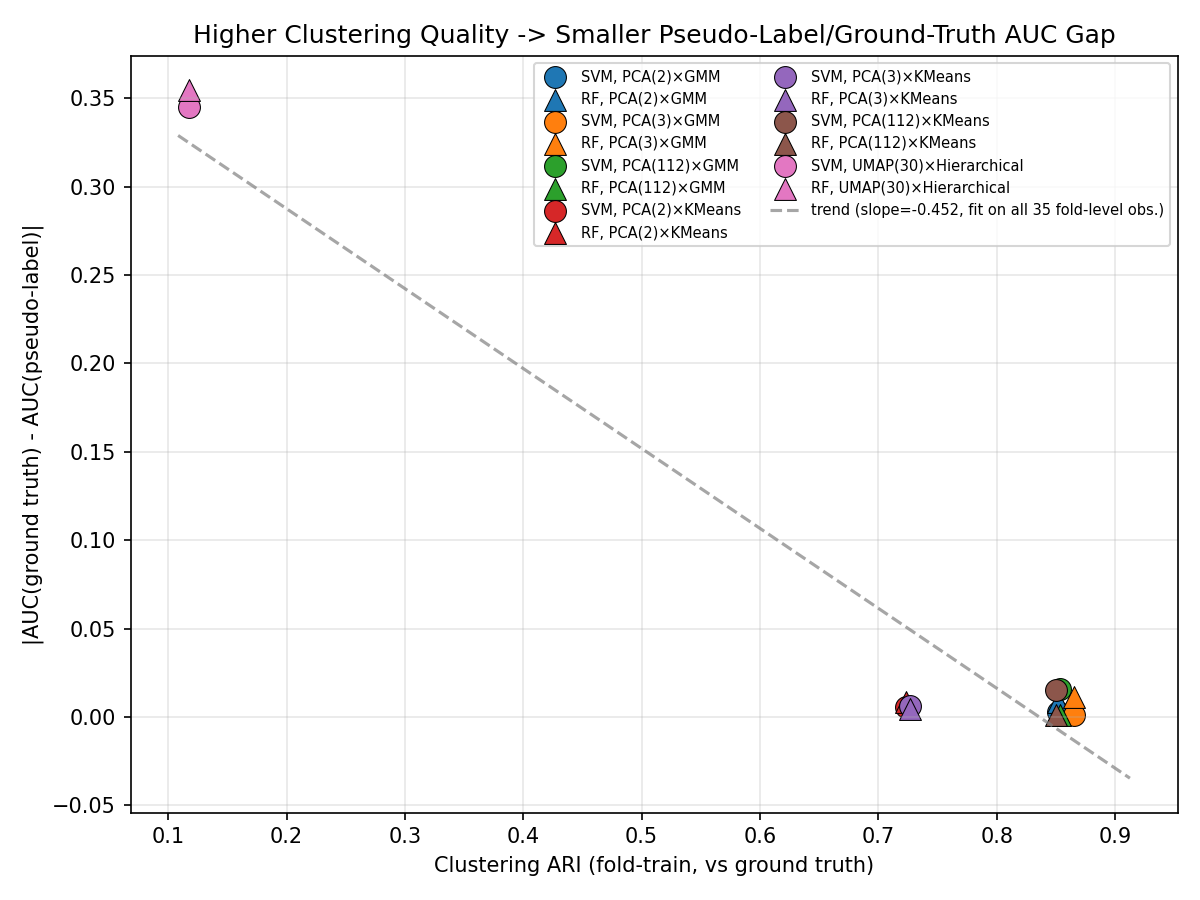
\includegraphics[width=\columnwidth]{images/cv_ari_vs_auc_gap_scatter.png}
\caption{Clustering ARI vs.\ absolute AUC gap (pseudo-label classifier minus ground-truth classifier). Each point is the mean across the 5 CV folds for one configuration/model (per-fold std is in Table~\ref{tab:cv}); the correlation ($r=-0.93$ SVM, $r=-0.94$ RF) is computed on the underlying 35 per-fold observations, not the plotted means.}
\label{fig:gap}
\Description{Scatter plot of Adjusted Rand Index against AUC gap showing one point per configuration and model, with a clear downward trend: high-ARI configurations cluster near zero gap, the low-ARI configuration shows a large gap.}
\end{figure}

This matters practically for validating a pipeline before deployment, but it requires computing ARI, which itself needs ground truth. This raises the natural follow-up question addressed next: can a fully label-free metric play the same role?

\subsection{Silhouette and Davies--Bouldin Do Not Substitute for ARI}
\label{sec:labelfree}
To test whether the relationship above could be operationalized with zero ground truth, we computed the silhouette score and Davies--Bouldin (DB) index -- both fully label-free -- for all eleven training-set clustering configurations (Table~\ref{tab:labelfree}). Neither correlates with ARI ($r=0.18$, $p=0.60$ for silhouette; $r=-0.17$, $p=0.63$ for DB): the configuration best by ARI (KMeans, $n=112$) is not best by silhouette (KMeans, $n=2$) or DB (Hierarchical, $n=2$). Table~\ref{tab:labelfree} shows why: silhouette and DB both degrade monotonically as dimensionality increases within every algorithm family -- a well-documented curse-of-dimensionality effect on distance-based internal validity indices -- whereas ARI does not, peaking at the highest dimensionality for KMeans. Distance-based label-free metrics are therefore not reliable substitutes for ARI here, and the ARI-vs-AUC-gap relationship (Section~\ref{sec:aritrust}) should be understood as a validation tool for settings where some labeled reference data is available -- e.g., a small annotated subset, or a previously labeled cohort -- rather than a fully label-free heuristic.

\textbf{The present study is itself positioned to serve as that reference cohort for future KIRC methylation work}: since our labeled data spans the same tissue type and Illumina 450K platform any new KIRC cohort would use, the ARI-vs-AUC-gap relationship established here can calibrate confidence in a pseudo-label classifier fit on new, unlabeled KIRC data, without re-deriving it from scratch. We confirm this transfer within the same TCGA-KIRC cohort in Section~\ref{sec:generalization} (holdout ARI $=0.8245$ vs.\ training $0.876$); extension to independent KIRC cohorts on the same platform is expected but not yet directly tested.

\begin{table}[t]
\caption{Label-free internal metrics vs.\ ARI (training set). Best value per column in bold; silhouette higher is better, DB lower is better.}
\label{tab:labelfree}
\resizebox{\columnwidth}{!}{%
\begin{tabular}{lccc}
\toprule
Configuration & ARI & Silhouette & Davies--Bouldin \\
\midrule
KMeans, $n=2$          & 0.749  & \textbf{0.452} & 0.812 \\
KMeans, $n=3$          & 0.786  & 0.377 & 0.973 \\
KMeans, $n=112$        & \textbf{0.876} & 0.111 & 2.150 \\
KMeans, raw            & $-$0.007 & 0.257 & 1.462 \\
Hierarchical, $n=2$    & 0.862  & 0.449 & \textbf{0.735} \\
Hierarchical, $n=3$    & 0.876  & 0.377 & 0.910 \\
Hierarchical, $n=112$  & 0.724  & 0.105 & 2.341 \\
Hierarchical, raw      & 0.811  & 0.070 & 2.710 \\
GMM, $n=2$             & 0.822  & 0.447 & 0.736 \\
GMM, $n=3$             & 0.848  & 0.361 & 0.892 \\
GMM, $n=112$ (diag.)   & 0.588  & 0.097 & 2.975 \\
\bottomrule
\end{tabular}}
\end{table}

\subsection{Generalization to Held-Out Samples}
\label{sec:generalization}
Applying the fitted PCA + KMeans pipeline (fit only on training data) to the untouched, patient-disjoint holdout set yields ARI $=0.8245$, close to the training ARI of $0.876$. This indicates the pipeline generalizes within the same cohort and platform. We stress that this is a same-cohort, same-platform validation; we have not tested transfer to an independent KIRC methylation cohort, and we make no claim that this specific PCA + clustering configuration is optimal for other cancer types, whose methylation architecture differs from KIRC's.

\section{Discussion}

Our results support three claims. First, dimensionality-reduction choice is not a stylistic detail but a decision with major empirical consequences: PCA's variance-maximizing objective matches a global, two-group separation task like tumor/normal status far better than UMAP's local-structure-preserving objective, and this should be verified empirically per task rather than assumed from UMAP's popularity in visualization contexts. Second, our AUCs ($\sim$0.99--1.00) are consistent with, not an outlier from, the supervised literature cited in Section~\ref{sec:intro} \cite{ding2019integrative, liu2019dna} -- our contribution is reaching comparable performance \emph{without any labels used in training}, notable given that KIRC-specific methylation literature has largely shifted toward prognosis \cite{tang2020novel} precisely because tumor/normal discrimination is already considered solved in the supervised regime. Third, and most importantly, the ARI-vs-AUC-gap relationship is a genuinely new, actionable heuristic, but with a boundary we tested directly rather than assumed: it requires ARI, and therefore some reference ground truth. Fully label-free internal metrics (silhouette, Davies--Bouldin) cannot remove that requirement in our setting. Practitioners should read our result as a recipe for validating an unsupervised pipeline against a small labeled reference sample, not as certifying trustworthiness with zero labels whatsoever.

\textbf{Limitations.} Our holdout validation is same-cohort and same-platform; independent-cohort transfer remains untested. The ARI-vs-gap relationship, while strong, used one deliberately poor clustering arm to widen the observed range -- a broader sweep of degradation modes would strengthen the correlation estimate further. Our pipeline is tuned for binary tumor/normal separation in KIRC specifically; other cancers or multi-class subtyping may favor different configurations.

\section{Conclusion}
We presented a fully unsupervised pipeline for TCGA-KIRC tumor/normal classification that avoids ground-truth labels during training, validated it against patient-grouped leakage safeguards and 5-fold cross-validation, and showed it performs within 0.005 AUC of a fully supervised classifier. Beyond this result, we demonstrated that PCA substantially outperforms UMAP for this task (mean ARI 0.79 vs.\ 0.07) and, most notably, that clustering quality (ARI) strongly predicts the performance penalty of using pseudo-labels instead of ground truth ($r=-0.93$ to $-0.94$) -- while fully label-free internal metrics (silhouette, Davies--Bouldin) cannot replace ARI in this role. This provides a practical basis for validating an unsupervised classification pipeline against a small labeled reference sample before trusting it on new, unlabeled data, directly useful wherever verified tumor/normal annotations are scarce or delayed, even if not fully absent.


\begin{acks}
The authors thank the TCGA Research Network and the Xena Hub project for providing public access to the methylation and clinical data used in this study. Code and analysis notebooks are available at \url{https://github.com/ich-bin-tyrone/epi-clusters}.
\end{acks}

\begin{thebibliography}{9}

\bibitem{hubert1985comparing}
Lawrence Hubert and Phipps Arabie. 1985.
\newblock Comparing partitions.
\newblock \emph{Journal of Classification} 2, 1 (1985), 193--218.

\bibitem{mcinnes2018umap}
Leland McInnes, John Healy, and James Melville. 2018.
\newblock UMAP: Uniform Manifold Approximation and Projection for Dimension Reduction.
\newblock \emph{arXiv preprint arXiv:1802.03426} (2018).

\bibitem{jain2010clustering}
Anil K. Jain. 2010.
\newblock Data clustering: 50 years beyond K-means.
\newblock \emph{Pattern Recognition Letters} 31, 8 (2010), 651--666.

\bibitem{cortes1995support}
Corinna Cortes and Vladimir Vapnik. 1995.
\newblock Support-vector networks.
\newblock \emph{Machine Learning} 20, 3 (1995), 273--297.

\bibitem{breiman2001random}
Leo Breiman. 2001.
\newblock Random forests.
\newblock \emph{Machine Learning} 45, 1 (2001), 5--32.

\bibitem{ding2019integrative}
Wenbin Ding, Gang Chen, and Tingming Shi. 2019.
\newblock Integrative analysis identifies potential DNA methylation biomarkers for pan-cancer diagnosis and prognosis.
\newblock \emph{Epigenetics} 14, 1 (2019), 67--80.

\bibitem{liu2019dna}
Biao Liu, Yulu Liu, Xingxin Pan, Mengyao Li, Shuang Yang, and Shuai Cheng Li. 2019.
\newblock DNA Methylation Markers for Pan-Cancer Prediction by Deep Learning.
\newblock \emph{Genes} 10, 10 (2019), 778.

\bibitem{tang2020novel}
Weihao Tang, Yiling Cao, and Xiaoke Ma. 2020.
\newblock Novel prognostic prediction model constructed through machine learning on the basis of methylation-driven genes in kidney renal clear cell carcinoma.
\newblock \emph{Bioscience Reports} 40, 7 (2020), BSR20201604.

\end{thebibliography}

\end{document}
